\section{Experiment Environment}

\begin{figure}[htbp]
\centering
  \begin{minipage}[h]{0.45\linewidth}
    \centering
    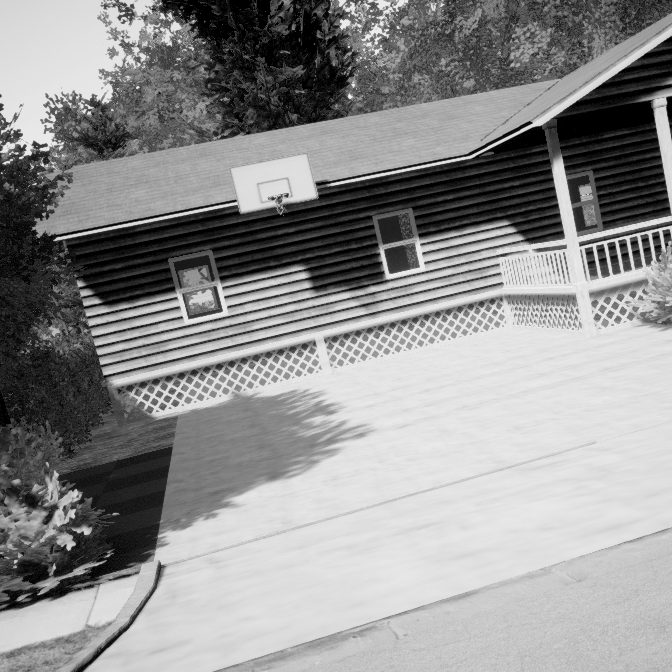
\includegraphics[keepaspectratio, scale=0.11]{./figure/3_environment/image10_0.png}
    \subcaption{Camera Image}\label{fig:known_env_image}
  \end{minipage} 
  \begin{minipage}[h]{0.45\linewidth}
    \centering
    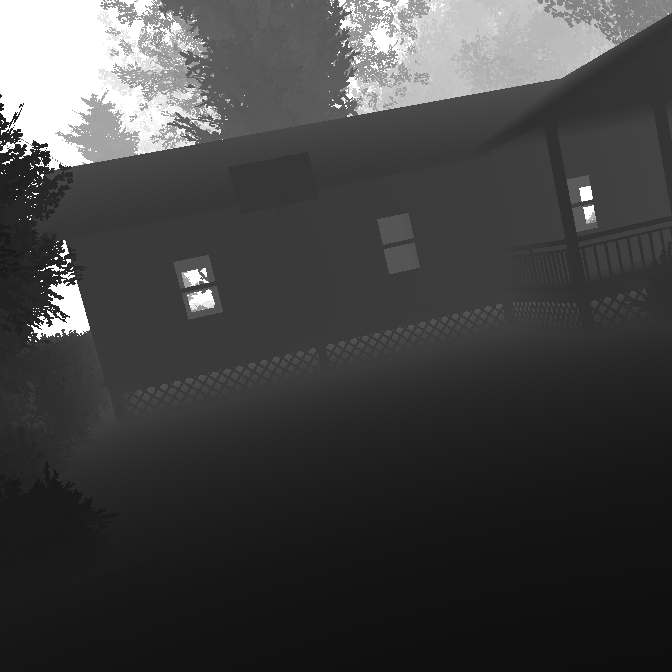
\includegraphics[keepaspectratio, scale=0.11]{./figure/3_environment/depth10_0.png}
    \subcaption{Depth Image}
  \end{minipage}
  \caption{Images Obtained from the Known Environment}\label{fig:known_env}
\end{figure}

\begin{figure}[thpb]
\centering
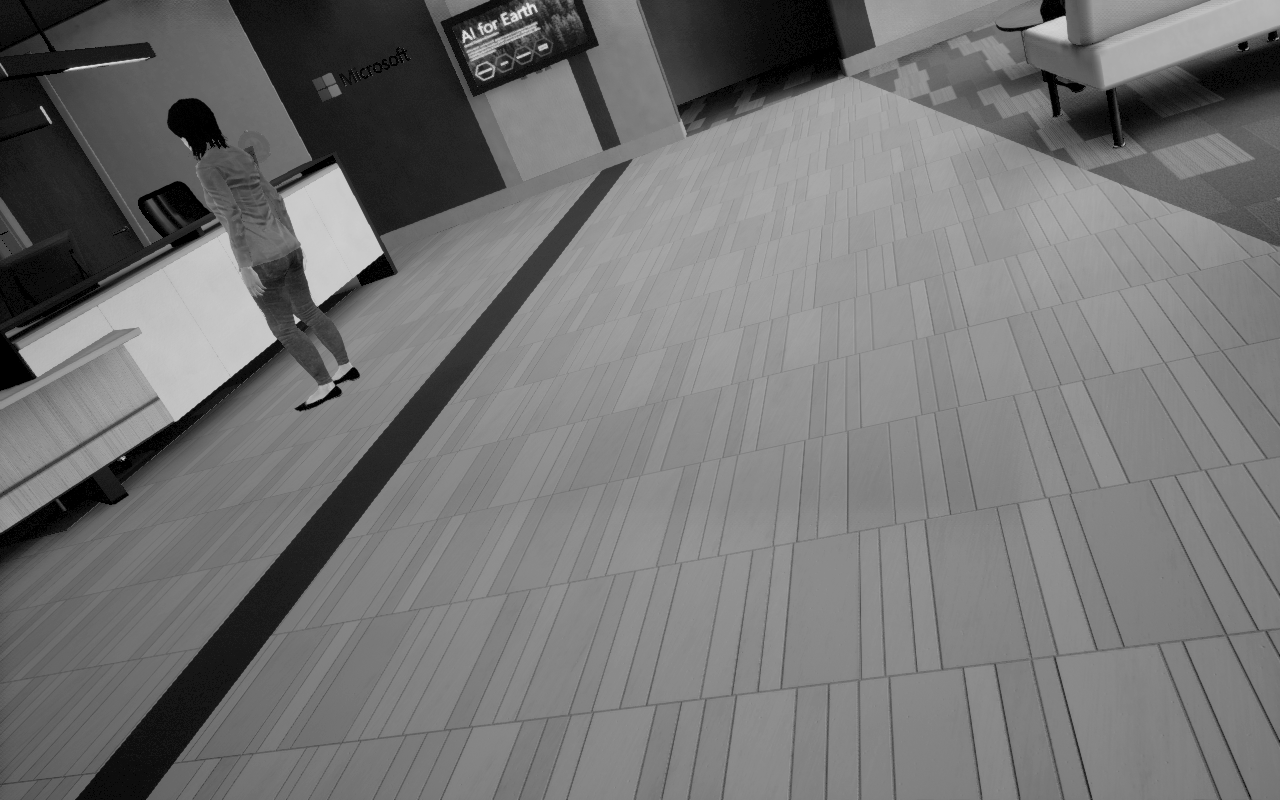
\includegraphics[scale=0.08]{./figure/3_environment/image64.png}
\caption{Image Obtained in Unknown Environment}
\label{fig:unknown_env}
\end{figure}

\subsection{Dataset Collection}\label{sec:dataset}
Microsoft AirSim\cite{airsim_paper} was used to collect data. This software is a drone simulator, but it can collect various data related to the task of attitude estimation, such as depth image collection. The drone spawned at random locations and collected images and attitude data as seen from those locations. To maximize the effectiveness of the method described in Sec.\ref{sec:random_window}, we modified the method to collect about five small images from a single location. In addition, images were collected from two environments for data collection. One environment was a suburban residential area with a moderate presence of trees and buildings. The images obtained in this environment were used for training and validation data and as part of the test data. The other environment was a Microsoft office building. Images obtained from this environment were not used for training data at all but were used as test data to measure performance in the environment in which the findings were obtained. Based on the above rules, 150,000 pairs of camera and depth images for training, 25,000 pairs for validation, and 1,000 pairs for testing were collected from the residential area environment described above. In addition, 1,000 pairs were collected from the office building environment described above for testing in the findings environment. The environment used to collect data for training is shown in Fig.\ref{fig:known_env}, and the environment used to collect data in an unknown environment is shown in Fig.\ref{fig:unknown_env}. The training and test images were grayscaled to compress data size and speed up processing. However, when inference is used, the number of channels is 3 to make it a pre-trained ResNet input. In a real environment, images obtained from a depth camera are subject to significant noise. However, in this study, in order to verify the effectiveness of using both the camera image and the depth image, we decided not to add noise information in the simulator environment. When trying to collect image and attitude data in a real environment, there is the problem of difficulty in obtaining accurate attitude values. Therefore, this experiment was conducted only in the simulator environment.

%データセットの収集にはMicrosoft AirSimを使用した。このソフトはドローンのシミュレータであるが, depth画像の採取などattitude estimationのタスクに関わる様々なデータが採取できる。実験データの採取では、ドローンをランダムな位置にスポーンさせてその位置から見たcamera imageとdepth image、そしてattitude dataを採取する方法を取った。また、Sec. AAAで紹介した手法の効果を最大限高めるため、一つの地点から小画像を5枚ほど採取するように変更した。また、データ採取にあたって2つの環境から画像を採取した。一つは郊外の住宅街をもした環境であり、木や建物などが適度に存在する。この環境下で得られた画像はtrainとvalidation用のデータと、testデータの一部に使用した。もう一つはマイクロソフト社のオフィスビルをもした環境であり、この環境から得られた画像は訓練用データには一切使用せず、所見の環境でのパフォーマンスを図るtest用のデータとして使用した。以上のルールに基づいて、訓練用のcamera imageとdepth imageを15万ペア、validation用として5万ペア、test用として1000ペアを先述の住宅街の環境から採取した。また、所見の環境でのテストのために先述のオフィスビルの環境から1000ペアを採取した。データサイズの圧縮と、処理の高速化のために訓練用の画像とテスト用の画像はグレイスケール化を行った.ただし、inferenceの時はpretrainedなResNetのinputとするためにチャネル数を3で読み込む.実環境においてdepthカメラから得られる画像には大きなノイズが発生する。しかし、本研究においてはcamera imageとdepth imageの2つを使うことの有効性を検証するために、シミュレータ環境におけるノイズ情報は付与しないことにした。


\subsection{Hardware}
%i9-10900K 32GB RTX2080Ti
%Nvidia DGX1
In this experiment, different hardware was used for learning and inference. We used NVIDIA DGX-1 for training, Intel core i9-10900K 10 cores 20 threads, 32GB RAM, and GeForce NVIDIA RTX2080Ti GPU for inference.

%今回の実験では学習と推論で異なるハードウェアを使用した。学習にはNvidia社製のDGX1を使用、推論にはIntel core i9-10900K 10コア20スレッド、RAMは32GB、GPUにはNvidia RTX2080Tiを使用した。




\subsection{Comparison Method}
Kawai's method\cite{9708864} and Ozaki's method\cite{Ozaki_SII2021} (MLE, Regression) were trained and tested as comparison methods. To examine the effect of the SA-Gate, we trained and tested a network without the SA-Gate from the network with the best experimental results in the proposed method in sec.\ref{sec:result}.

\begin{table}[htbp]
\begin{center}
\caption{Training Parameter}
  \begin{tabular}{c|c} \hline
    Parameter & Value \\ \hline
    Learning Loss & 1e-4 \\
    Mean Element & 0.5 \\
    Std Element & 0.5 \\
    Epochs & 50 \\
    Batch Size & 256 \\
    Dropout Rate & 0.1 \\
    L2 Regularization Alpha & 5e-5 \\
    Optimizer & Adam \\
    Loss Function & Cross Entropy Loss \\ \hline
  \end{tabular}
  \label{tab:Training_Parameter}
\end{center}
\end{table}

\subsection{Train Network}
The hyperparameters used in the train are shown in Tab.\ref{tab:Training_Parameter}. During training, 8 GPUs were parallelized for training. Pytorch is used for the implementation. The feature extractor in the proposed method can be equipped with ResNet of any layer depth. ResNet was trained using 18, 34, 50, 101, and 152 as feature extractor, respectively. It took about 50 hours to complete the training. 
%Train is shown in Fig\ref{fig:train_network}.

%提案手法におけるfeature extractorは任意の層の深さのResNetを搭載することができる。本実験ではResNet18, 34, 50, 101, 152それぞれで学習を行い、推論試験を行った。Training graphを図AAAAに示す。学習が終了するまでの時間は概ね50時間ほどであった。

